\documentclass[a4paper, 12pt]{article}
\input{prefix_pension.tex}%
\newcommand{\Set}[2]{\left\{ #1 \;\middle\vert\; #2 \right\}}

\newcommand{\pth}[1]{\mleft(#1\mright)}%

\renewcommand{\P}{\operatorname{P}}
\newcommand{\E}{\operatorname{E}}
\newcommand{\Var}{\operatorname{Var}}
\newcommand{\Cov}{\operatorname{Cov}}
\newcommand{\diam}[1]{\operatorname{diam}\mleft(#1\mright)}
\newcommand{\osc}[2]{\operatorname{osc}\mleft(#1,\, #2\mright)}
\newcommand{\supp}[1]{\operatorname{supp}\mleft(#1\mright)}
\newcommand{\indicator}{\mathbf{1}}
\newcommand{\argmin}{\operatorname{argmin}}
\newcommand{\argmax}{\operatorname{argmax}}
\newcommand{\deq}{\stackrel{d}{=}}

\DeclareMathOperator*{\mtimes}{\text{\raisebox{0.25ex}{\scalebox{0.8}{$\bigtimes$}}}}
\DeclareMathOperator*{\motimes}{\text{\raisebox{0.25ex}{\scalebox{0.8}{$\bigotimes$}}}}

\newcommand{\Ex}[1]{\E\mleft[ #1 \mright]}

\newcommand{\ceil}[1]{\mleft\lceil {#1} \mright\rceil}
\newcommand{\floor}[1]{\mleft\lfloor {#1} \mright\rfloor}
\newcommand{\sgn}{\operatorname{sgn}}
\newcommand{\card}{\operatorname{card}}

\newcommand{\brc}[1]{\left\{ {#1} \right\}}
\newcommand{\sbrc}[1]{\left[ {#1} \right]}
\newcommand{\set}[1]{\brc{#1}}%

\newcommand{\abs}[1]{\left\lvert {#1} \right\rvert}%
\newcommand{\norm}[1]{\left\lVert {#1} \right\rVert}
\newcommand{\spanby}{\operatorname{span}}
\newcommand{\esssup}{\operatorname{ess\,sup}}
\newcommand{\inp}[2]{\left\langle {#1},\, {#2} \right\rangle}

\newcommand{\mto}{\overset{m}{\to}}
\newcommand{\wto}{\overset{w}{\to}}
\newcommand{\wstarto}{\overset{w^*}{\to}}
\newcommand{\asto}{\overset{a.s.}{\to}}
\newcommand{\pto}{\overset{p}{\to}}
\newcommand{\dto}{\overset{d}{\to}}
\newcommand{\dsubset}{\overset{d}{\subset}}


\newcommand{\ds}{\displaystyle}%

\newcommand{\R}{\mathbb{R}}%
\newcommand{\N}{\mathbb{N}}
\newcommand{\Q}{\mathbb{Q}}
\newcommand{\Z}{\mathbb{Z}}
\newcommand{\C}{\mathbb{C}}
\newcommand{\F}{\mathcal{F}}
\newcommand{\A}{\mathcal{A}}
\newcommand{\B}{\mathcal{B}}
\newcommand{\T}{\mathcal{T}}
\newcommand{\M}{\mathcal{M}}
\newcommand{\V}{\mathcal{V}}
\renewcommand{\L}{\mathcal{L}}
\renewcommand{\S}{\mathcal{S}}
\newcommand{\I}{\mathcal{I}}
\renewcommand{\H}{\mathcal{H}}
\newcommand{\D}{\mathcal{D}}
\newcommand{\U}{\mathcal{U}}
\newcommand{\G}{\mathcal{G}}
\newcommand{\J}{\mathcal{J}}

\newcommand{\one}{\mathbf{1}}

\newcommand{\exist}{\exists\:}
\newcommand{\forany}{\forall\:}
\renewcommand{\ae}{\quad\text{a.e.}}
\newcommand{\Res}{\operatorname{Res}}
\newcommand{\cl}{\operatorname{cl}}

\newcommand{\iidsim}{\overset{iid}{\sim}}
\newcommand{\Poisson}{\text{Poisson}}
\newcommand{\Ber}{\text{Ber}}
\newcommand{\Exp}{\text{Exp}}

\newcommand{\restrict}[1]{\left.\hspace{-0.2em}\right|_{#1}}
\newcommand{\eval}[3]{\left.{#1}\right|_{#2}^{#3}}

% derivatives
\makeatletter
\renewcommand\d[1]{\mspace{6mu}\mathrm{d}#1\@ifnextchar\d{\mspace{-3mu}}{}}
\makeatother
\def\at{
  \left.
  \vphantom{\int}
  \right|
}

\newcommand{\od}[2]{\frac{d{#1}}{d{#2}}}
\newcommand{\odd}[2]{\frac{d^2{#1}}{d{#2}^2}}
\newcommand{\pd}[2]{\frac{\partial{#1}}{\partial{#2}}}
\newcommand{\pdd}[2]{\frac{\partial^2{#1}}{\partial{#2}^2}}
\newcommand{\pdpd}[3]{\frac{\partial^2{#1}}{\partial{#2}\partial{#3}}}

\makeatletter
\newcommand*{\rom}[1]{\expandafter\@slowromancap\romannumeral #1@}
\makeatother

\title{Pension Run}

\author{Kai-Jyun Wang}

\begin{document} 
\setstretch{1.15}

\maketitle

\section{Introduction}
Why do retirees give up longevity insurance? In the canonical life-cycle model,
an individual who faces an uncertain lifetime should convert a substantial share
of wealth into an annuity. Pooling mortality risk allows an annuity to sustain
consumption for as long as the retiree lives, a protection that self-insurance
cannot provide as cheaply \citep{yaari1965,davidoff2005}. Yet observed
annuitization is limited: even when retirees are offered a direct choice between
a lump-sum benefit and a stream of lifetime payments, many choose the lump sum.
This gap between the theoretical value of longevity insurance and actual choices
is the annuitization puzzle \citep{brown2008,benartzi2011}.

Most explanations of the puzzle treat the value of the promised annuity as
independent of other retirees' choices. That assumption is natural for an
actuarially fair contract backed by a solvent insurer, but it is less innocuous
for benefits paid by a financially vulnerable pension fund. A lifetime payment
is valuable only while the provider remains able and willing to pay. When a fund
is expected to become depleted, the effective maturity of its monthly benefit is
shortened. A retiree may then rationally prefer an immediate lump sum even when
the scheduled, undiscounted value of monthly benefits is larger. Low
annuitization can therefore reflect not only preferences for liquidity or
bequests, but also exposure to provider-solvency risk.

The central tension is that the annuity is the more generous option if all
promised payments are honored, yet its generosity can undermine the promise
itself. When early cohorts choose monthly benefits, they build a persistent stock
of long-lived liabilities. In the environment we study, those obligations
eventually deplete the fund, whereas the fund remains sustainable if every
generation instead takes the less generous lump-sum benefit. Insolvency is
therefore not simply an exogenous reason to avoid annuitization; it can be the
equilibrium consequence of earlier cohorts accepting the annuity offer.

This intergenerational feedback gives the pension run two stages. Early
recipients choose the more valuable monthly benefit and gradually weaken the
fund's solvency. Once the accumulated obligations make depletion sufficiently
likely, later retirees discount the promised stream and switch toward immediate
lump-sum claims. These large current withdrawals can bring depletion forward and
further reduce the value of annuitization. We call this feedback a \emph{pension
run}. Unlike a standard bank run, retirees do not withdraw identical demandable
claims at the same time. They make a one-time choice as they retire, so aggregate
fragility develops through a sequence of benefit-maturity decisions across
generations.

This paper develops a continuous-time model of that mechanism. New retirees
choose between an immediate lump-sum payment and a life-contingent monthly
benefit. Their choice depends on the present value of monthly payments, which in
turn depends on the stochastic time at which the pension fund is depleted.
Individual choices determine both current withdrawals and the stock of monthly
beneficiaries, feeding back into the fund's dynamics and its bankruptcy time.
The equilibrium is summarized by a nonlinear valuation equation linking the
fund balance, outstanding pension liabilities, annuity demand, and solvency.
The framework thus turns one possible explanation of the annuitization puzzle
into an equilibrium source of pension-system fragility.

\paragraph{Related literature.}
This paper contributes first to the literature on annuity demand. The benchmark
result is that households facing uncertain lifetimes value annuities because
they insure consumption against longevity risk \citep{yaari1965,davidoff2005}.
Observed behavior falls well short of this benchmark. Using U.S. Health and
Retirement Study data, \citet{brown2001} finds that the life-cycle value of an
annuity predicts whether defined-contribution balances are annuitized, but leaves
much of the observed choice unexplained. \citet{dushi2004} likewise document very
low purchases of additional annuities among older U.S. households. Evidence from
the United Kingdom also shows limited participation in the voluntary annuity
market \citep{inkmann2011}. Even when an annuity is offered directly within a
pension plan, a substantial minority takes cash: in U.S. pension data,
\citet{hurd2006} find that 20 percent of benefits offering a lump-sum option are
cashed out. Taken together, these studies establish a persistent gap between the
large theoretical gains from longevity insurance and retirees' willingness to
annuitize, although its magnitude varies with the institutional setting
\citep{benartzi2011}.

The literature offers several explanations for this gap. Adverse selection
raises the price and lowers the money's worth of voluntary annuities because
individuals with private information that they are long-lived are more likely to
purchase them \citep{finkelstein2002}. Fixed nominal annuities expose retirees to
inflation risk, while inflation-indexed products have historically been scarce
in private markets \citep{brown2002inflation}. Public pensions and
defined-benefit plans also pre-annuitize a large share of household wealth,
reducing the marginal value of purchasing additional longevity insurance
\citep{dushi2004}. Health and medical-expense shocks create a separate demand for
liquid wealth. When high medical costs are correlated with changes in mortality,
the remaining value of an annuity can be especially low precisely when those
expenses arise \citep{reichling2015}. Bequest motives, other liquidity needs, and
the framing of annuity products provide additional explanations
\citep{brown2008}.

Most closely related to our mechanism, \citet{hui2021} show that real and
perceived provider-insolvency risk, together with imperfect information about
guaranty protection, can substantially reduce annuity demand and welfare. In
their analysis, households take the provider's insolvency risk as given when
choosing how much to annuitize. In our setting, insolvency is endogenous:
retirees' choices between lump-sum and monthly benefits alter the fund's cash
flows and hence its probability of depletion. Annuity demand, provider solvency,
and the value of the annuity are therefore jointly determined in equilibrium.

Second, the paper relates to research on the sustainability and reform of public
pensions. Demographic aging erodes the contribution base and expands benefit
obligations, creating adjustments in taxes, benefits, retirement ages, labor
supply, and private saving \citep{attanasio2007,boerschsupan2016}. Structural
analyses quantify how pension institutions and reforms reshape retirement and
life-cycle decisions \citep{french2011,kitao2018,daminato2024,delalibera2026}.
Our focus is complementary. We hold the principal policy parameters fixed and
ask how a benefit-withdrawal option can propagate financial stress even before a
reform occurs. This introduces beneficiary composition---the division of new
retirees between immediate and deferred claims---as an endogenous determinant of
pension solvency.

Relatedly, our mechanism connects to evidence that retirement decisions respond
to expectations about future pension policy. \citet{huixin2023} show that the
timing of pension retrenchments matters: immediately implemented reforms delay
retirement, whereas reforms announced with long implementation lags can bring
retirement forward, particularly when the reform is fundamental or trust in
government is low. We likewise emphasize forward-looking responses to the
credibility of future benefits. In our setting, however, the relevant uncertainty
arises endogenously from the fund's financial state, and retirees' responses feed
back into that state rather than merely responding to an externally specified
reform path.

Finally, the paper is related to models of runs and maturity choice. The classic
bank-run literature shows how individually optimal withdrawals can generate
aggregate fragility \citep{diamond1983,goldstein2005}. The closest structural
analogue is the dynamic debt-run model of \citet{he2012}, in which creditors arrive
sequentially and decide whether to roll over maturing short-term debt. We retain
the stochastic fundamental, staggered decisions, and endogenous default time,
but the underlying claim is different. A retiree chooses once between an
immediate payment and a life-contingent stream; this choice changes both current
outflows and the evolving stock of monthly-benefit recipients. The pension run
therefore operates through endogenous benefit maturity and demographic turnover,
rather than repeated rollover of fixed-maturity debt.

\section{Institutional Background}
\subsection{Labor Insurance old-age benefits}
The empirical setting is the old-age benefit provided by Taiwan's Labor
Insurance program. This social-insurance benefit is distinct from the Labor
Pension system, under which employers contribute to workers' individual
retirement accounts. Labor Insurance is financed collectively by premiums and
the assets of the Labor Insurance Fund, and benefits are administered by the
Bureau of Labor Insurance (BLI).

An old-age pension was introduced on January 1, 2009. An insured worker with at
least 15 years of coverage may claim a monthly pension after leaving employment
and reaching the statutory claim age. The statutory age increased gradually
from 60 and reaches 65 in 2026. A worker may claim up to five years early or
defer for up to five years; the monthly benefit is reduced or increased by 4
percent for each year. At the normal claim age, the BLI pays the larger amount
implied by
\begin{equation}\label{eq:taiwan_annuity}
    p = \max\left\{0.00775\,wY+3{,}000,\;
                    0.0155\,wY\right\},
\end{equation}
where $w$ is the average of the worker's highest 60 monthly insured salaries and
$Y$ is years of coverage.

The 2009 reform created the choice studied in this paper. Workers with any Labor
Insurance coverage before December 31, 2008 may choose either the monthly
pension or the pre-reform \emph{one-time old-age benefit}; the choice is
irreversible once the BLI approves and pays the claim. Workers first insured in
2009 or later cannot choose the pre-reform benefit. The
one-time benefit generally pays one month of average insured salary for each of
the first 15 coverage years and two months for each additional year, subject to
a ceiling of 45 months before age 60 and 50 months including post-60 coverage.
This grandfathered payment is the lump sum in our model. It should not be
confused with the separately defined \emph{old-age lump-sum benefit} for workers
with fewer than 15 years of coverage, whom we exclude from the choice sample.

The statutory formulas make the annuity potentially much more generous than the
lump sum. For example, a worker with an average insured salary of NT\$45,800 and
30 years of coverage receives NT\$2.061 million under the one-time formula but
NT\$21,297 per month under the second formula in \cref{eq:taiwan_annuity}. If the
worker receives the pension for 12 years, its present value at a 2 percent annual
discount rate is approximately NT\$2.72 million. The monthly option therefore
offers valuable longevity insurance as well as a larger expected transfer, but
it also creates a persistent liability for the common fund. This difference is
the institutional basis for the tradeoff in our model.

Taiwan's government has made direct budgetary contributions to the Labor
Insurance Fund since 2020. Accordingly, ``bankruptcy'' in the model
does not mean that current law mechanically terminates benefits when recorded
assets reach zero. It denotes exhaustion of the fund under existing contribution
and benefit rules---the point at which continued payment requires an additional
fiscal transfer or a reform. The baseline estimation ends in December 2019 to
identify the fund's endogenous dynamics before regular government injections;
the later observations remain useful for describing choices and validating the
entry reconstruction.

\section{Data}
\subsection{Sources and sample construction}
We construct a monthly panel beginning in January 2009, when the old-age pension
was introduced. The current data vintage ends in June 2026, the latest month for
which all component series are available. The panel combines three official
sources. First, monthly reports from the Bureau of Labor Funds (BLF) provide the
exact month-end balance and investment return of the Labor Insurance Fund. We
read the balance from the report's asset-allocation table rather than its rounded
narrative total. The fund included both ordinary and occupational-accident
insurance through April 2022; following the institutional separation in May
2022, the reported Labor Insurance Fund contains only ordinary insurance.
Second, BLI statistical tables provide the stock of
old-age-pension recipients, pension recipients receiving their first payment,
and claims for the one-time old-age benefit.
Third, Ministry of the Interior (MOI) population files provide monthly registered
population and annual population and deaths by age.

We retain only one-time old-age benefit claims as lump-sum choices. In
particular, we exclude the old-age lump-sum benefit for short coverage histories
and the old-age difference payment because neither represents the same choice
between the grandfathered lump sum and the monthly pension. Let $L_t$ denote the
number of qualifying one-time claims in month $t$, $Q_t$ the stock of monthly
pension recipients, and $A_t$ the number entering the monthly scheme. The
empirical monthly-choice share is
\begin{equation}\label{eq:data_q}
    q_t = \frac{A_t}{A_t+L_t}.
\end{equation}
The two state variables used in estimation are the fund balance per registered
resident, $B_t/N_t$, and monthly pension recipients per resident, $Q_t/N_t$.

\subsection{Reconstructing entries into the monthly scheme}
The BLI reports $Q_t$ throughout the sample, but identifies first-payment
recipients only from May 2022 onward. A change in $Q_t$ is not itself an entry
measure because recipients leave the stock when they die. For the earlier
period, we reconstruct monthly entries from the accounting identity
\begin{equation}\label{eq:entry_reconstruction}
    \widehat A_t
    = \max\left\{0,\;Q_t-Q_{t-1}+\delta_t Q_{t-1}+c\right\},
\end{equation}
where $\delta_t$ is the monthly mortality probability for Taiwan residents aged
60 and older. We calculate the corresponding annual death probability from MOI
age-specific deaths and population, then convert it to a monthly probability as
$1-(1-d_t)^{1/12}$. If the current year's age table has not yet been released,
we carry forward the latest available annual rate.

The constant $c$ corrects for systematic differences between the stock-flow
identity and reported first payments. We estimate it over the post-May-2022
overlap as the mean of $A_t-(Q_t-Q_{t-1}+\delta_tQ_{t-1})$. In the current data
vintage, the overlap contains 50 months and yields $c=-2{,}452.84$ recipients per
month; the mean absolute reconstruction error in that validation period is 179
recipients. We use reported first payments whenever they are available and the
adjusted reconstruction beforehand. Equation \eqref{eq:entry_reconstruction}
assumes that mortality is the only exit from the recipient stock and applies the
mortality of all residents aged 60 and older to Labor Insurance beneficiaries.
The reconstructed early series should therefore be interpreted as a measurement
of annuity entry rather than an exact administrative count.

\begin{figure}[t]
    \centering
    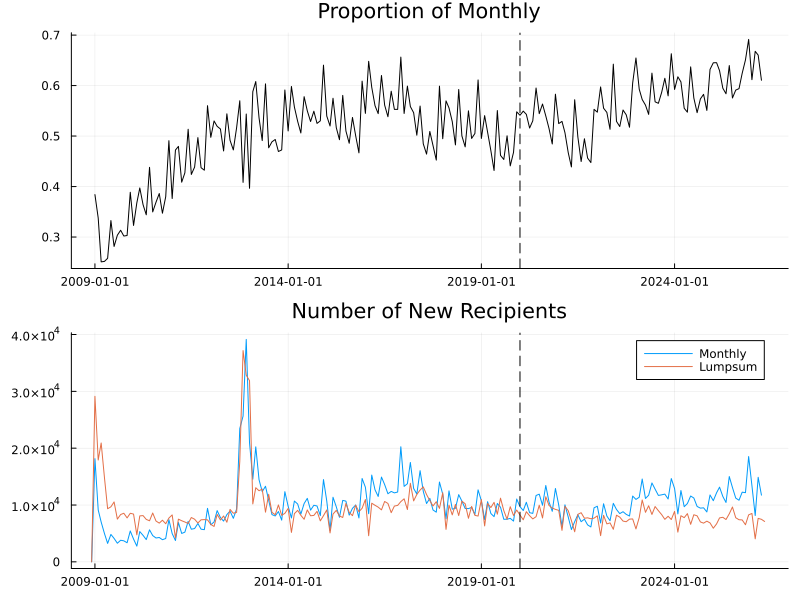
\includegraphics[width=0.72\textwidth]{../figure/recipients.png}
    \caption{New Labor Insurance old-age benefit recipients}
    \label{fig:recipients}
\end{figure}

\section{Model}
We consider a continuous time model with an infinite horizon. There is a continuum 
of individuals choosing between the lumpsum and the monthly pension schemes. The 
pension fund is running by the government with the return and the volatility being 
exogenously given. When the pension system goes bankrupt, the recipients cannot 
receive any more pensions from then on. 

\subsection{Population}
Let $b(s), m(s)$ be the fertility rate and the mortality rate respectively. 
Let $g(t,s)$ be the unnormalized population density. The population dynamic 
is given by 
\begin{equation}
    \pd{g}{t} = -\underbrace{\pd{g}{s}}_{\text{aging}} - \underbrace{mg}_{\text{mortality}} + \underbrace{\int bgds\delta_0}_{\text{birth}}
\end{equation}
where $\delta_0$ denotes the Dirac delta centered at $0$. To simplify the 
model, we take the assumptions that $b(s) = b$ is a constant and that 
$m(s) = m\one\set{s\geq T_m}$. In plain words, this means that only those 
who have aged $T_m$ exposes to the mortality risks.\footnote{We recognize 
that this is a somewhat restrictive and unrealistic assumption, but as we 
are going to see, this assumption helps to greatly simplify the computation.}

Let $N_t = \int_0^\infty g(t, s)ds$ be the total population and $\hat{g}(t, s)
= \frac{g(t, s)}{N_t}$ be the normalized population density. Assuming that $\hat{g}$ 
is at its steady state, an analytical solution is available: 
\begin{equation}
    \hat{g}(s) = \begin{cases}
        be^{-ns}, & s < T_m \\ 
        be^{-ns}e^{-m(s-T_m)} & s\geq T_m
    \end{cases}
\end{equation}
where $n = \frac{\dot{N}_t}{N_t}$ is the population growth rate satisfying
\begin{equation}
    1 = b\frac{1 - e^{-nT_m}}{n} + be^{-nT_m}\frac{1}{n+m}.
\end{equation}
For a detailed derivation, we refer to \cref{app:pop_eqs}. 

\subsection{Pension System}
We assume that all households retire at age $T$. When retiring, the households 
choose between a lumpsum transfer $\ell$ and a monthly pension that pays a stream 
of income $p$. Let $\mathcal{Q}(t, s)$ be the population density among the monthly pension 
recipients. The dynamic is given by 
\begin{equation}
    \pd{\mathcal{Q}}{t} = -\underbrace{\pd{\mathcal{Q}}{s}}_{\text{aging}} - \underbrace{m\mathcal{Q}}_{\text{mortality}} + \underbrace{q_t\hat{g}(T)N_t\delta_T}_{\text{new retirees}}
\end{equation} 
where $q_t$ is the proportion of new retirees choosing pension. Suppose that 
$T\geq T_m$. We can further simplify the recipients dynamic thanks to our 
assumption on the mortality rate. Let $Q_t = \int_T^\infty \mathcal{Q}(t, s)ds$. 
$Q_t$ follows the law of motion 
\begin{equation}
    dQ_t = \sbrc{q_t\hat{g}(T)N_t - mQ_t}dt. 
\end{equation}  

Let $B_t$ be the level of the pension fund. Its law of motion is given by 
\begin{equation}
    dB_t = \sbrc{\underbrace{rB_t}_{\text{interest}} + \underbrace{\tau yN_t\int_{T_w}^T\hat{g}(s)ds}_{\text{pension tax}} - \underbrace{(1-q_t)\ell N_t\hat{g}(T)}_{\text{lumpsum}} - \underbrace{pQ_t}_{\text{monthly}}}dt + \sigma B_tdZ_t,  
\end{equation}
where $Z_t$ is a Brownian motion. $\tau$ is the tax rate; $y$ is the income 
; $T_w$ is the age when individuals start to work. 

The system goes bankrupt when $B_t$ hits $0$. Denote the remaining 
time for $B_t$ to hit $0$ by $T_B$. We shall consider the detrended states 
$\hat{B}_t = \frac{B_t}{N_t}, \hat{Q}_t = \frac{Q_t}{N_t}$. 
Since $N_t$ is positive in finite time, the bankrupt time 
is equivalent to the time when $\hat{B}_t = 0$. In other words, 
the the remaining time for $\hat{B}_t$ hitting $0$, $T_{\hat{B}}$, coincides 
with $T_{B}$. The law of motions for the transformed states are given by 
\begin{align}\label{eq:state_dynamic}
    d\hat{B}_t &= \sbrc{(r-n)\hat{B}_t + \tau y\int_{T_w}^T\hat{g}(s)ds - (1-q_t)\hat{g}(T)\ell - p\hat{Q}_t}dt + \sigma\hat{B}_tdZ_t \\
    d\hat{Q}_t &= \sbrc{q_t\hat{g}(T)-(m+n)\hat{Q}_t}dt. 
\end{align}
To simplify the notation, we also denote the drift terms 
by $\mu_B$ and $\mu_Q$, respectively.

\subsection{Individuals' Pension Decisions}
A retiring individual $i$ chooses between between the two 
schemes $d\in\set{\ell, p}$ to maximize the utility, given by  
\begin{equation}
    u_{it}(d) = \begin{cases}
        \alpha + \log(\ell) + \epsilon_i(\ell) &\text{if } d = \ell, \\
        \log(V_t) + \epsilon_i(p) &\text{if } d = p,
    \end{cases}
\end{equation}
where $V_t$ is the present discount value of the monthly pension 
given the current states $(\hat{B}_t, \hat{Q}_t)$, 
\begin{equation}\label{eq:value}
    V_t = V(\hat{B}_t, \hat{Q}_t) = \E\sbrc{\int_0^{T_{\hat{B}}} e^{-(\rho+m)s}pds\:\bigg|\: \hat{B}_t, \hat{Q}_t}
\end{equation}
with $\rho$ being the subjective discount factor. We assume that 
the $\epsilon_i(d)$ are independent and identically 
distributed across individuals and the choices, following the 
standard Gumbel distribution. The shift parameter $\alpha$ controls 
the preference of the lumpsum scheme over the monthly one. Although 
we do not model here elaborately, this may be thought to represent 
the need of liquidity or the incomplete pension market. Another 
parameter $\beta$ controls the sensitivity to the flucutation in 
the present discount value of the monthly pension.  

By the property of the Gumbel distribution, the individuals' choices 
aggregate to the proportion choosing the monthly scheme 
\begin{equation}\label{eq:aggregation}
    q_t = \P_t(u_{it}(p)>u_{it}(\ell)) = \frac{1}{1+\exp\pth{\alpha + \log(\ell) - \log(V_t)}}
\end{equation}
by the law of large number across the individuals. Note that 
$q_t$ is a function of $\hat{B}_t$ and $\hat{Q}_t$ since 
$V_t = V(\hat{B}_t, \hat{Q}_t)$. 

\subsection{Equilibrium}
We now list down the equilibrium conditions. Given the Markovian 
states $(\hat{B}_t, \hat{Q}_t)$, the equilibrium is determined 
by the present discount value of the monthly pension $V_t$ and 
the proportion choosing monthly shceme $q_t$ such that 
\begin{thmenum}
    \item Given $q_t$, the law of motions of the states $(\hat{B}_t, \hat{Q}_t)$ 
    is consistent with $q_t$ (\cref{eq:state_dynamic}).
    \item Given the law of motions of the states, the present 
    discount value of the monthly pension $V(\hat{B}_t, \hat{Q}_t)$ 
    is consistent with the law of motions (\cref{eq:value}). 
    \item The individuals optimize and the decisions aggregate 
    to $q_t$ (\cref{eq:aggregation}). 
\end{thmenum}

To determine the equilibrium, it suffices to compute $V(\hat{B}, \hat{Q})$. 
Notice that $V$ satisfies the following Hamilton-Jacobi-Bellman equation 
\begin{equation}
    (\rho + m)V = p + \A V, 
\end{equation}
with the boundary condition $V(0, \hat{Q}) = 0$ for all 
$\hat{Q}$. The operator 
\begin{equation}
    \A f = \mu_B\pd{f}{B} + \mu_Q\pd{f}{Q} + \frac{1}{2}\sigma^2B^2\pdd{f}{B}
\end{equation}
is the infinitesimal generator. Since the the drift terms 
also depend on $V$, this partial differential equation is 
nonlinear. 

To solve the model numerically, we impose the artificial 
boundary at the upper bound of $\hat{B}$. Since clearly $V_t$ 
has upper bound $\frac{p}{\rho+m}$ and is increasing in $\hat{B}$, 
it follows that $\pd{V}{B}$ is approximately $0$ for $\hat{B}$ 
sufficiently large.

We solve the model based on the finite difference method alongside 
the successive iteraiton that shares the same spirit with Howard's policy 
iteration method. This numerical scheme can be viewed as an semi-implicit 
scheme with time step size being infinite. The sparsity of the generator 
matrix is exploited to achieve a better efficiency. We present our 
algorithm explicitly in \cref{alg:successive_iteration}. 
\begin{algorithm}[ht]
    \caption{Successive Iteration}
    \label{alg:successive_iteration}
    
\begin{algorithmic}[1]
\Require Initial guess $V^{(0)}$, tolerance $\epsilon>0$, maximum iterations $K$
\State Set $k \gets 0$
\Repeat
    \State Given $V^{(k)}$, compute 
    \begin{equation*}
        \mu_B^{(k)} = \mu_B(B, Q, V^{(k)}(B, Q)), \quad \mu_Q^{(k)} = \mu_Q(B, Q, V^{(k)}(B, Q))
    \end{equation*}
    and the infinitesimal generator 
    \begin{equation*}
        \A^{(k)} = \mu_B^{(k)}\pd{}{B} + \mu_Q^{(k)}\pd{}{Q} + \frac{1}{2}\sigma^2B^2\pdd{}{B}.
    \end{equation*}
    with adjustments to the boundary nodes. 
    \State Solve the linear system 
    \begin{equation*}
        \pth{(\rho+m)I - \A^{(k)}}V^{(k+1)} = \mathbf{b}, \quad 
        \mathbf{b} = p\operatorname{vec}\begin{pmatrix}
            0 & 0 & \cdots & 0 \\ 
            1 & 1 & \cdots & 1 \\ 
            \vdots & \ddots & \ddots & \vdots \\ 
            1 & \cdots & 1 & 1
        \end{pmatrix}.
    \end{equation*}
    \State Compute the error 
    \begin{equation*}
        e^{(k+1)} \gets \norm{V^{(k+1)} - V^{(k)}}_\infty.
    \end{equation*}
    \State $k \gets k+1$
\Until{$e^{(k)}<\epsilon$ or $k=K$}
\State \Return $V^{(k)}$. 
\end{algorithmic}

\end{algorithm}


\section{Results}
\subsection{Calibration}
We separate the parameters in the model in to two parts. One is calibrated outside the 
model and the other is estimated by solving the inverse problem. To illustrate the estimation 
procedure, denote the estimand vector $\theta$. The data is a time series 
$X_i = (\hat{B}_i, \hat{Q}_i)$ sampled from equidistant time grids of gap size $\Delta$. 

The parameters for the population structure are calibrated to Taiwan's 
population. We take $T_m = T_r = 65$ and $T_w = 20$. The birth rate is set to 
be the total fertility rate in 2025 and the mortality rate leads to the median 
lifespan being $77$. The details are given in \cref{tab:parameters}. 

\begin{table}[ht]
    \centering
    \caption{Model Parameters}
    \label{tab:parameters}
    \vspace{0.5em}
    \begin{threeparttable}
    \begin{tabular}{clcl}
        \toprule
        Parameter & Description & Value & Target \\
        \midrule
        \multicolumn{4}{l}{\textit{Panel A: External Calibration}} \\
        \addlinespace
        $b$ & Birth rate & $0.00462$ & Total fertility rate \\
        $m$ & Mortality rate & $0.06$ & Median lifespan \\
        $T_w$ & Working age & $25$ &  \\
        $T_r$ & Retirement age & $61$ & Standard retirement age \\
        $T_m$ & Age of mortality exposure & $60$ &  \\
        $\rho$ & Subjective discount rate & $0.02$ & Interest rate \\
        $\tau$ & Pension tax & $0.075$ & Pension tax \\
        $y$ & Income & $5.268$ & Highest monthly insured salary \\
        $\ell$ & Lump-sum pension & $19.75$ & Transfer based on 30 years of working \\
        $p$ & Monthly pension & $2.449$ & Pension based on 30 years of working \\
        \addlinespace
        \midrule
        \multicolumn{4}{l}{\textit{Panel B: Internal Calibration}} \\
        \addlinespace
        $r$ & Pension fund return rate & $0.2686$ & $\E\sbrc{\frac{\hat{B}_{t+\Delta}-\hat{B}_t}{B_t}-\mu_{B}(\hat{B}_t, \hat{Q}_t, \theta)\Delta} = 0$ \\
        $\sigma$ & Pension fund volatility & $1.855$ & $\text{SD}(\frac{\hat{B}_{t+\Delta}-\hat{B}_t}{B_t\sqrt{\Delta}}) = \sigma$ \\
        $\alpha$ & Preference for lump-sum scheme & $-17.43$ & $\E\sbrc{(q - q(\hat{B}_t, \hat{Q}_t, \theta))^2}$ \\
        $\beta$ & Sensitivity to default risk & $0.6663$ & $\E\sbrc{(q - q(\hat{B}_t, \hat{Q}_t, \theta))^2}$ \\
        \bottomrule
    \end{tabular}

    \begin{tablenotes}[flushleft]
        \footnotesize
        \item \textit{Note:} The monetary unit in the model is 100,000 NTD.
    \end{tablenotes}
\end{threeparttable}

\end{table}

\begin{figure}[ht]
    \centering 
    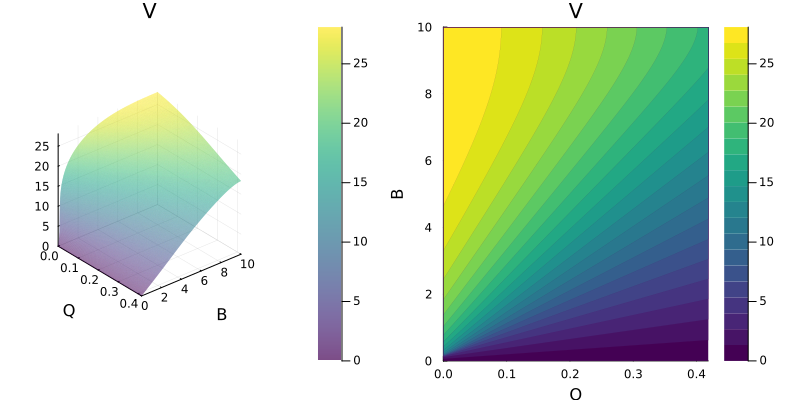
\includegraphics[scale=0.5]{../figure/estimated_V.png}
    \label{fig:estimated_V}
    \caption{Estimated $V$}
\end{figure}

\section*{Appendix}
\appendix
\section{Derivation of the Population Equations}\label{app:pop_eqs}
To find the steady state $\hat{g}$, conjecture that $g(t, s) = \hat{g}(s)N_t$. 
Plugging back to the population equation gives 
\begin{equation}
    \hat{g}(s)\frac{\dot{N}_t}{N_t} = -\pd{\hat{g}}{s} - m(s)\hat{g}(s) + b\delta_0. 
\end{equation}
Notice that the right hand side does not depend on $t$. Hence $\frac{\dot{N}_t}{N_t} = n$ 
is a constant. We can also write the Dirac delta as part of the boundary condition: 
\begin{equation}
    \hat{g}(s)n = -\pd{\hat{g}}{s} - m(s)\hat{g}(s), \quad 
    \hat{g}(0) = b. 
\end{equation}
This is a standard initial value problem with $m(s) = m$ for $s \geq T_m$ and $0$ 
otherwise. The solution is given by 
\begin{equation}
    \hat{g}(s) = \begin{cases}
        be^{-ns}, & s < T_m \\ 
        be^{-ns}e^{-m(s-T_m)} & s\geq T_m. 
    \end{cases}
\end{equation}
Finally, the population growth rate $n$ can be determined by the normalizing condition  
\begin{equation}
    \int_0^\infty \hat{g}(s)ds = 1\quad \Rightarrow\quad 1 = b\frac{1 - e^{-nT_m}}{n} + be^{-nT_m}\frac{1}{n+m}.
\end{equation}


\bibliographystyle{apacite}
\bibliography{pension}
\end{document}
